\documentclass[12pt]{report}
\usepackage[utf8]{inputenc}
\usepackage[russian]{babel}
%\usepackage[14pt]{extsizes}
\usepackage{listings}
\usepackage{graphicx}
\usepackage{amsmath,amsfonts,amssymb,amsthm,mathtools} 
\usepackage{pgfplots}
\usepackage{filecontents}
\usepackage{indentfirst}
\usepackage{eucal}
\usepackage{enumitem}
\frenchspacing

\usepackage{indentfirst} % Красная строка


\usetikzlibrary{datavisualization}
\usetikzlibrary{datavisualization.formats.functions}

\usepackage{amsmath}

% Для листинга кода:
\usepackage{caption}
\DeclareCaptionFont{white}{\color{white}}
\DeclareCaptionFormat{listing}{\colorbox{white}{\parbox{\textwidth}{#1#2#3}}}
\captionsetup[lstlisting]{format=listing,justification=raggedright}

\lstset{
	language=C,                 % выбор языка для подсветки
	basicstyle=\small\sffamily, % размер и начертание шрифта для подсветки кода
	numbers=left,               % где поставить нумерацию строк (слева\справа)
	numberstyle=\tiny,           % размер шрифта для номеров строк
	stepnumber=1,                   % размер шага между двумя номерами строк
	numbersep=5pt,                % как далеко отстоят номера строк от подсвечиваемого кода
	showspaces=false,            % показывать или нет пробелы специальными отступами
	showstringspaces=false,      % показывать или нет пробелы в строках
	showtabs=false,             % показывать или нет табуляцию в строках
	frame=single,              % рисовать рамку вокруг кода
	tabsize=2,                 % размер табуляции по умолчанию равен 2 пробелам
	captionpos=t,              % позиция заголовка вверху [t] или внизу [b] 
	breaklines=true,           % автоматически переносить строки (да\нет)
	breakatwhitespace=false, % переносить строки только если есть пробел
	escapeinside={\#*}{*)}   % если нужно добавить комментарии в коде
}

\usepackage[left=2cm,right=2cm, top=2cm,bottom=2cm,bindingoffset=0cm]{geometry}
% Для измененных титулов глав:
\usepackage{titlesec, blindtext, color} % подключаем нужные пакеты
\definecolor{gray75}{gray}{0.75} % определяем цвет
\newcommand{\hsp}{\hspace{20pt}} % длина линии в 20pt
% titleformat определяет стиль
\titleformat{\chapter}[hang]{\Huge\bfseries}{\thechapter\hsp\textcolor{gray75}{|}\hsp}{0pt}{\Huge\bfseries}


% plot
\usepackage{pgfplots}
\usepackage{filecontents}
\usetikzlibrary{datavisualization}
\usetikzlibrary{datavisualization.formats.functions}

\begin{document}
	\def\contentsname{Содержание}
	\def\refname{Список литературы}
	\thispagestyle{empty}
	\begin{titlepage}
		\noindent \begin{minipage}{0.15\textwidth}
			
\includegraphics[width=\linewidth]{b_logo}
		\end{minipage}
		\noindent\begin{minipage}{0.9\textwidth}\centering
			\textbf{Министерство науки и высшего образования Российской Федерации}\\
			\textbf{Федеральное государственное бюджетное образовательное учреждение высшего образования}\\
			\textbf{~~~«Московский государственный технический университет имени Н.Э.~Баумана}\\
			\textbf{(национальный исследовательский университет)»}\\
			\textbf{(МГТУ им. Н.Э.~Баумана)}
		\end{minipage}
		
		\noindent\rule{18cm}{3pt}
		\newline\newline
		\noindent ФАКУЛЬТЕТ $\underline{\text{«Информатика и системы управления»}}$ \newline\newline
		\noindent КАФЕДРА $\underline{\text{«Программное обеспечение ЭВМ и информационные технологии»}}$\newline\newline\newline\newline\newline
		
		
		\begin{center}
			\noindent\begin{minipage}{1.3\textwidth}\centering
				\Large\textbf{Домашнее задание}\newline
				\textbf{по дисциплине "Анализ алгоритмов"}\newline\newline
			\end{minipage}
		\end{center}
		
		\noindent\textbf{Тема} $\underline{\text{Графовые модели программ}}$\newline\newline
		\noindent\textbf{Студент} $\underline{\text{Петрова А. А. }}$\newline\newline
		\noindent\textbf{Группа} $\underline{\text{ИУ7-56Б}}$\newline\newline
		\noindent\textbf{Оценка (баллы)} $\underline{\text{~~~~~~~~~~~~~~~~~~~~~~~~~~~}}$\newline\newline
		\noindent\textbf{Преподаватели} $\underline{\text{Волкова Л.Л.}}$\newline\newline\newline
		
		\begin{center}
			\vfill
			Москва~---~\the\year
			~г.
		\end{center}
	\end{titlepage}
	
	
	\tableofcontents
	
	\newpage
	\chapter{Исходный код алгоритма}
	
	\begin{lstlisting}[label=some-code,caption=Функция быстрой сортировки массива целых чисел, language=C]
		void quick(int *mas, int size)
		{
			int i = 0;  // (1)
			int j = size - 1;  // (2)
			int mid = mas[size / 2];  // (3)
			do  // (4)
			{
				while (mas[i] < mid)  // (5)
					i++;  // (6)
				while (mas[j] > mid)  // (7)
					j--;  // (8)
				if (i <= j)  // (9)
				{
					int tmp = mas[i];  // (10)
					mas[i] = mas[j];  // (11)
					mas[j] = tmp;  // (12)
					i++;  // (13)
					j--;  // (14)
				}
			}
			while (i <= j);  // (4)
			if (j > 0)  // (15)
				quick(mas, j + 1);  // (16)
			if (i < size)  // (17)
				quick(&mas[i], size - i);  // (18)
		}
	\end{lstlisting}
	
	\chapter{Модели программ}
	
	\section{Граф управления программы}
	
	\begin{figure}[h]
		\centering
		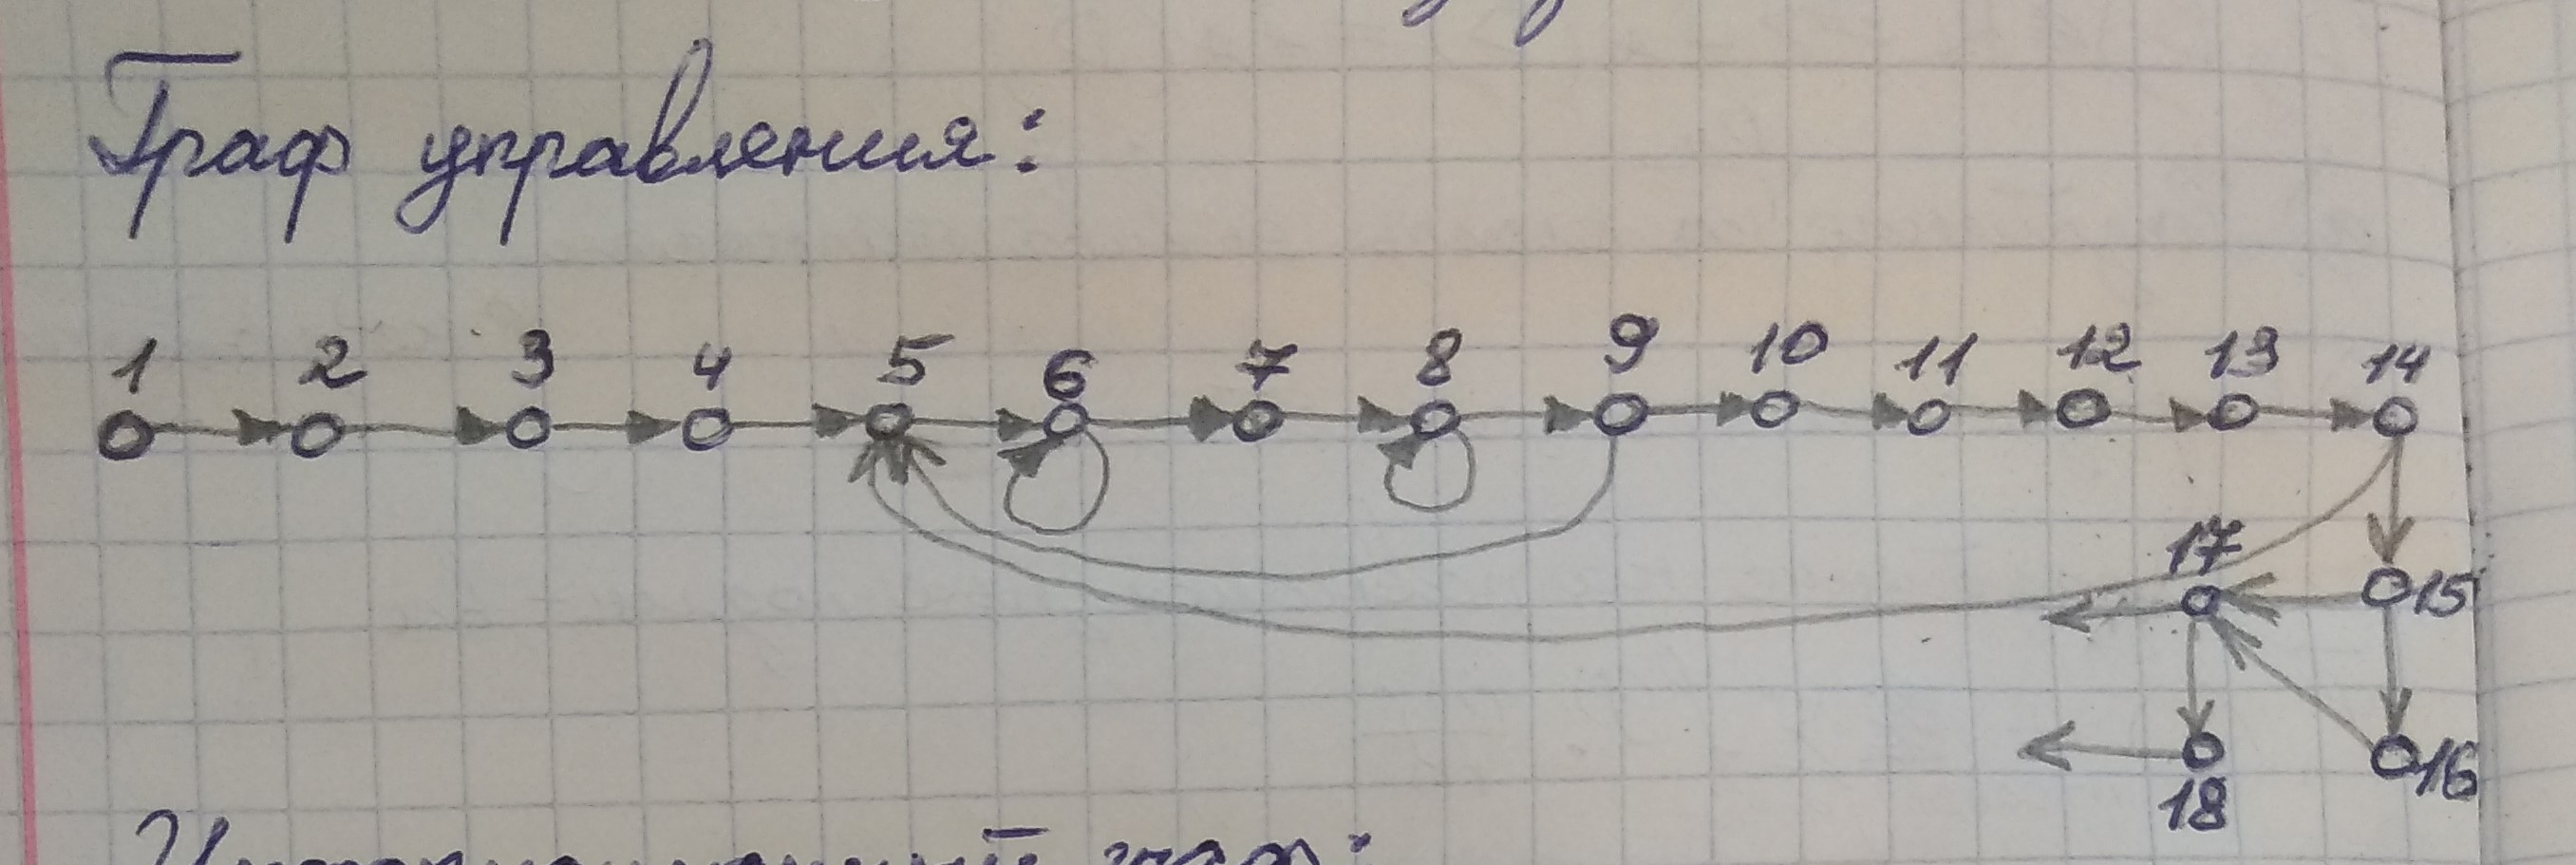
\includegraphics[scale=0.2]{control_graph.jpg}
		\caption{Граф управления программы}
		\label{fig:mpr}
	\end{figure}

	\newpage
	
	\section{Информационный граф программы}
	
	\begin{figure}[h]
		\centering
		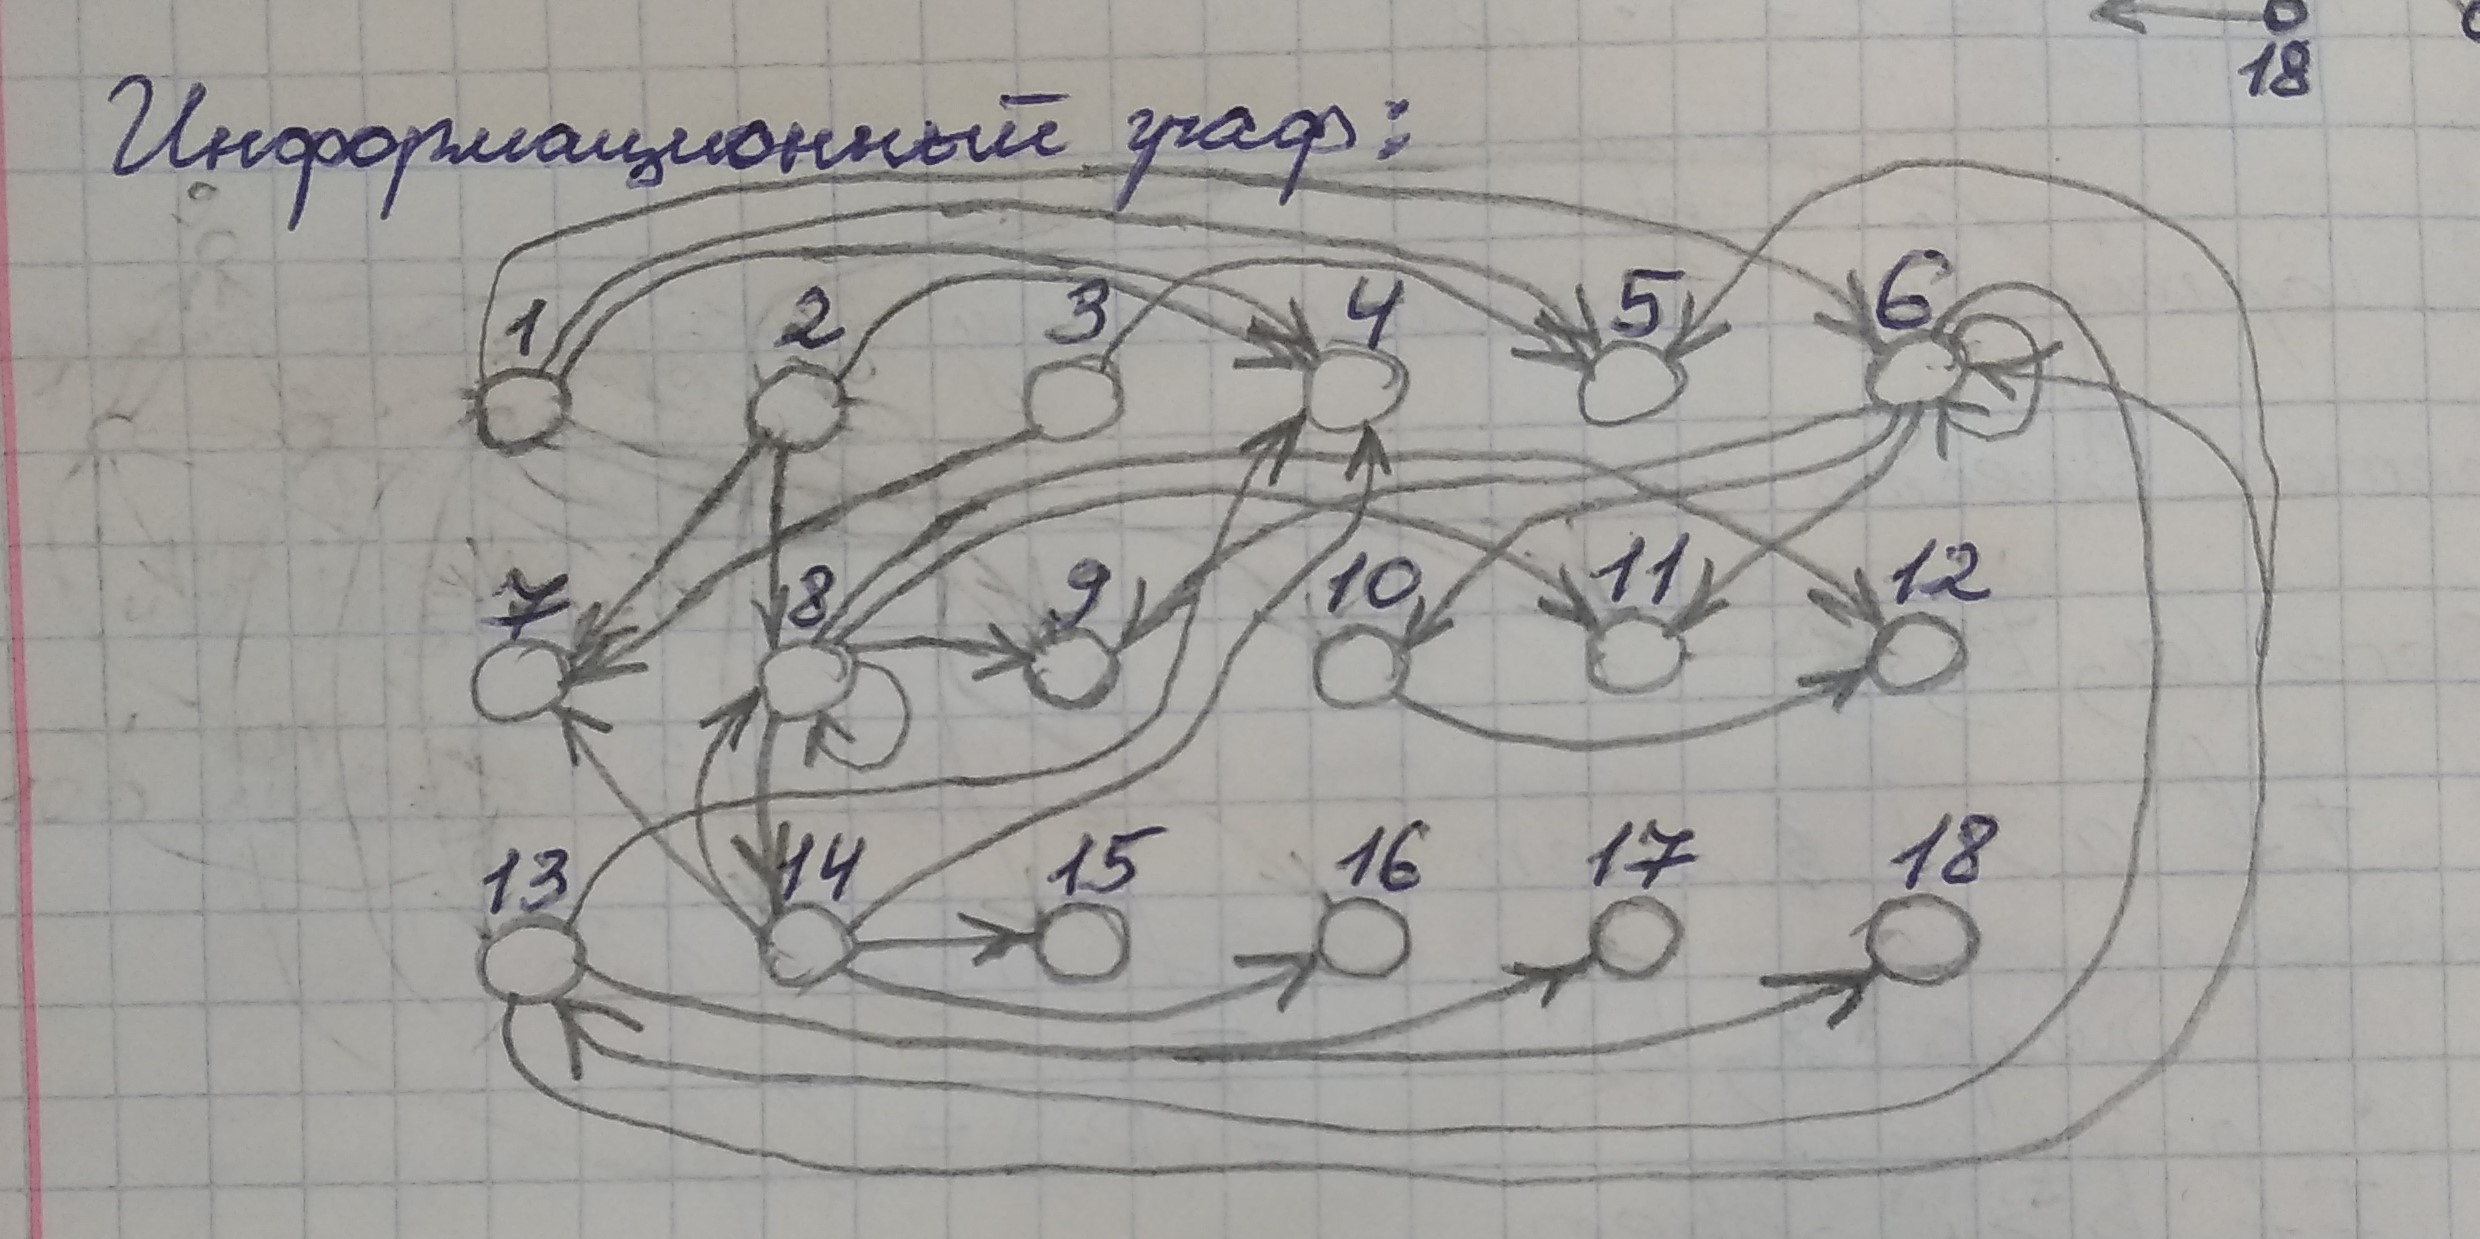
\includegraphics[scale=0.21]{inform_graph.jpg}
		\caption{Информационный граф программы}
		\label{fig:mpr}
	\end{figure}

	\newpage
	
	\section{Операционная история программы}
	
	Для конкретного массива [54, 26, 93, 17, 77] (в таком случае все if "сработают").
	
	\begin{figure}[h]
		\centering
		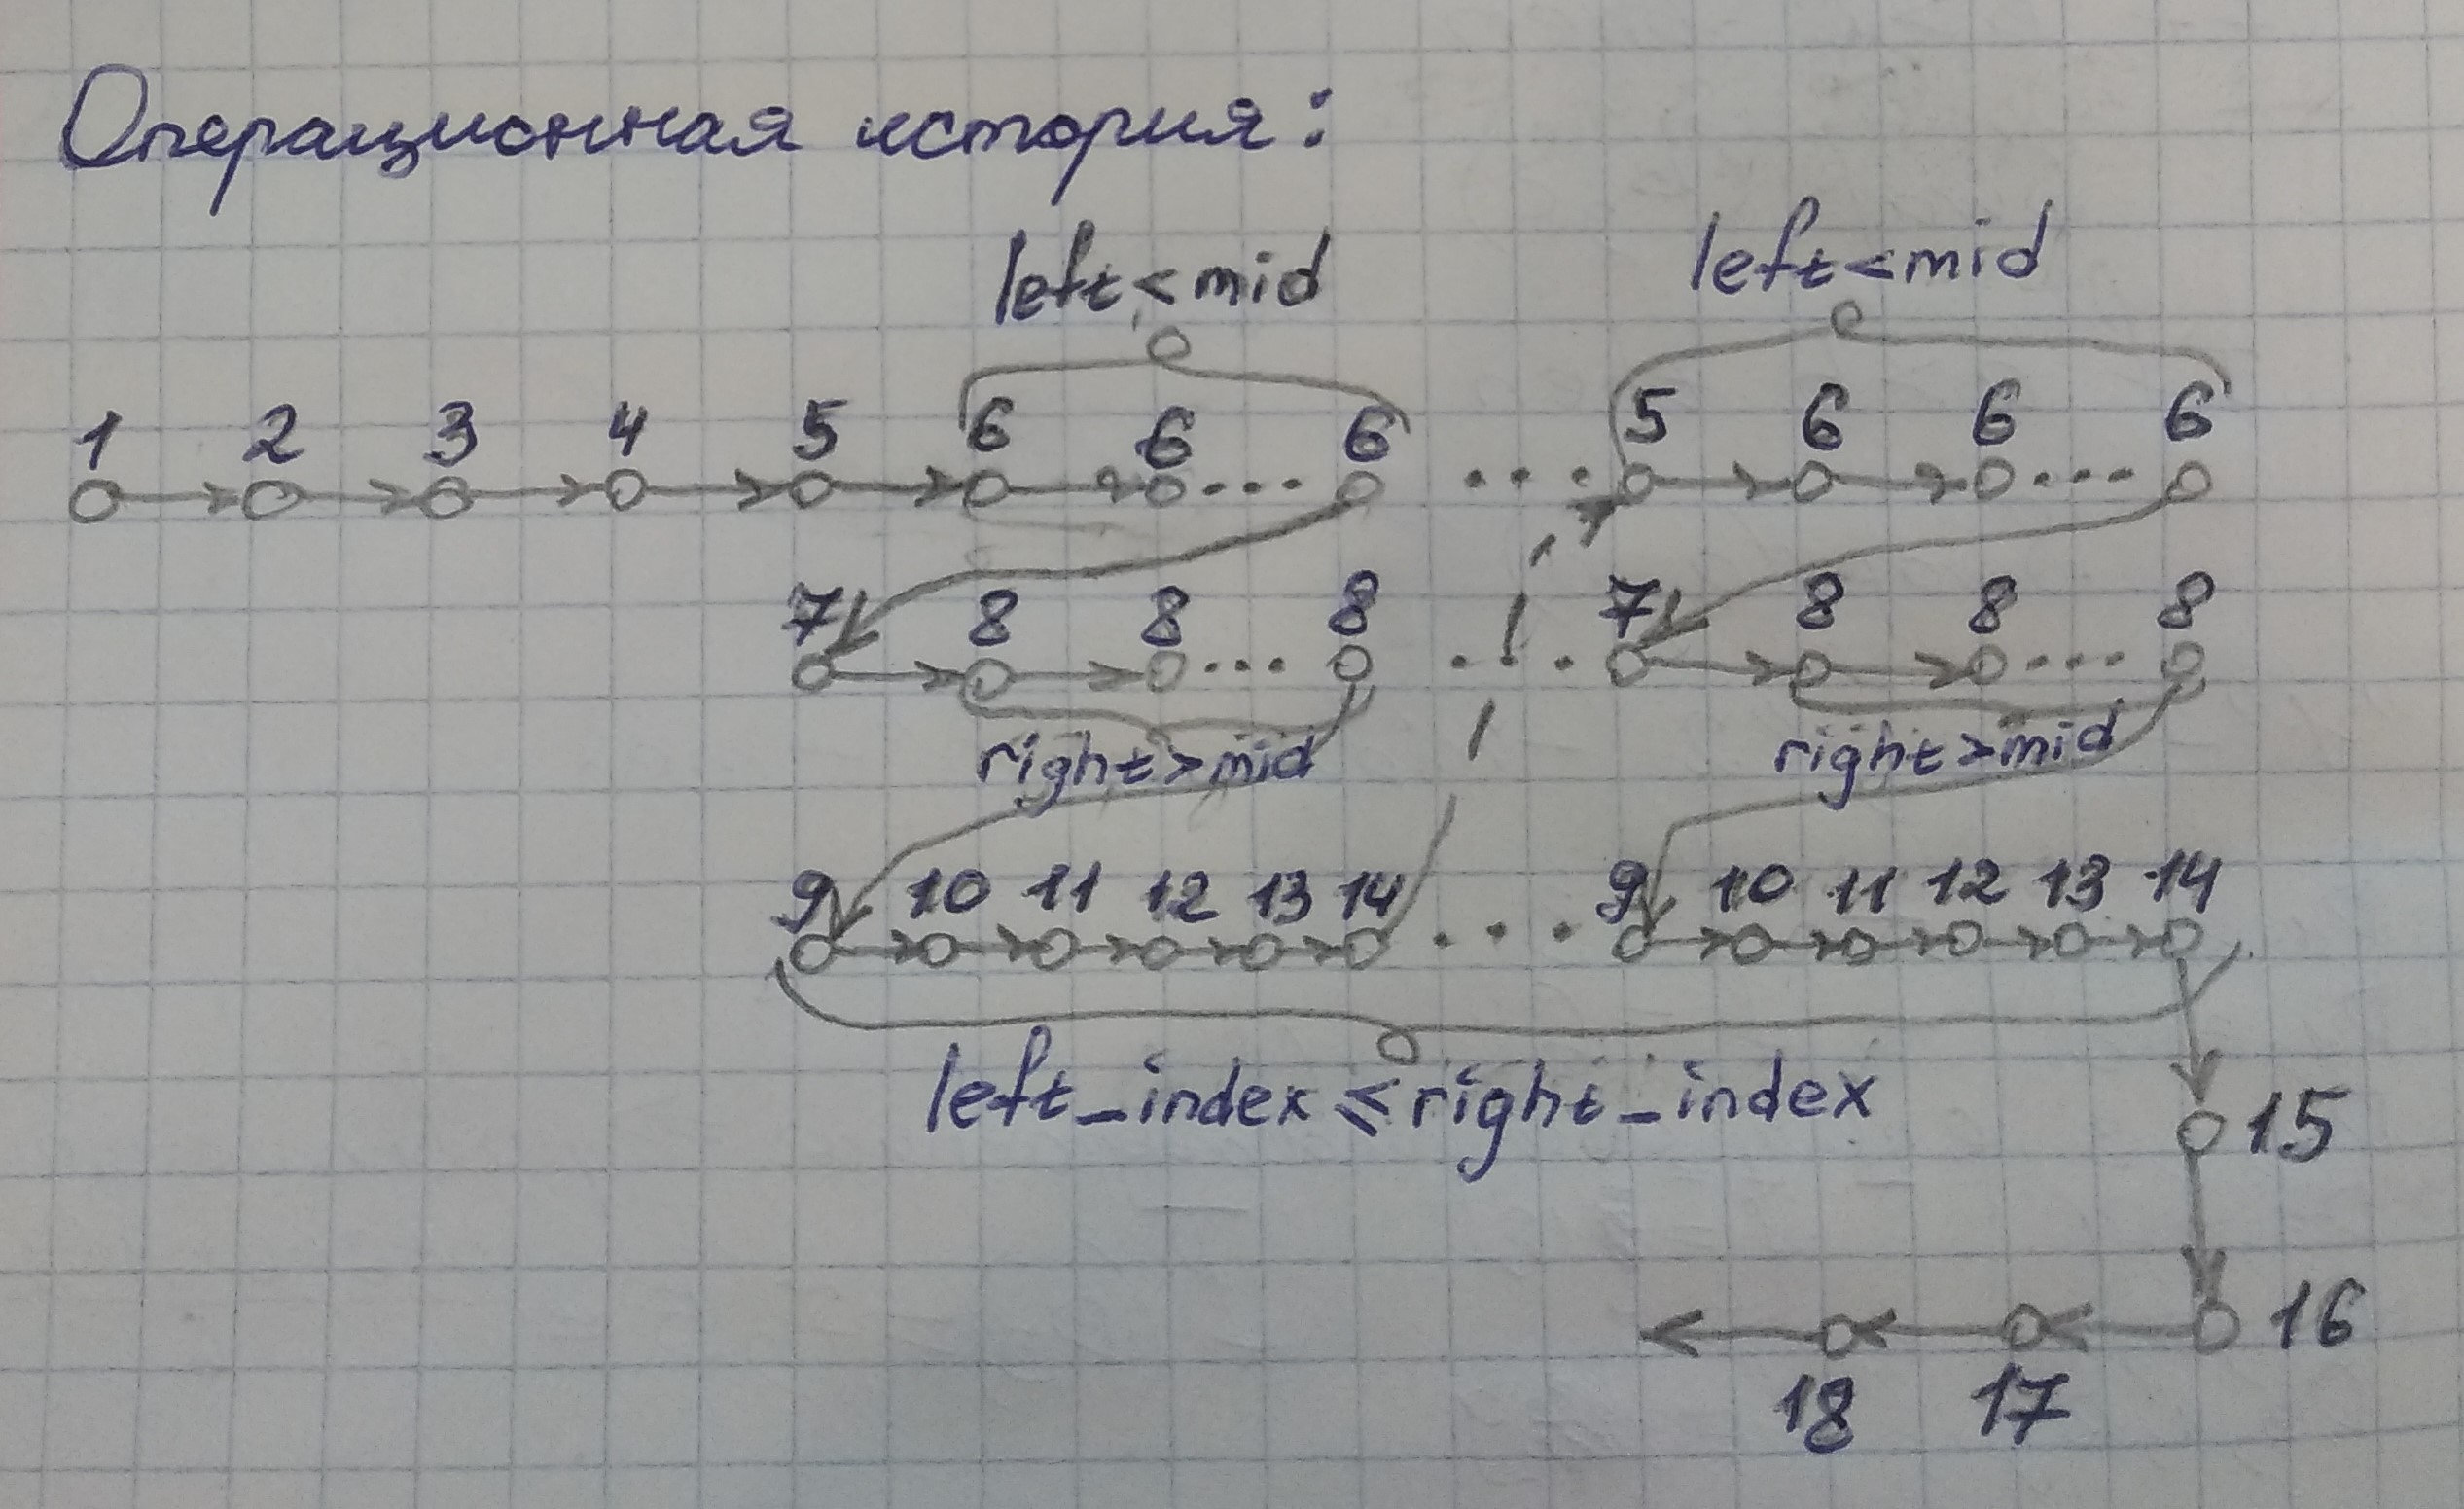
\includegraphics[scale=0.2]{oper_history.jpg}
		\caption{Операционная история программы}
		\label{fig:mpr}
	\end{figure}

	\newpage
	
	\section{Информационная история программы}
	
	\begin{figure}[h]
		\centering
		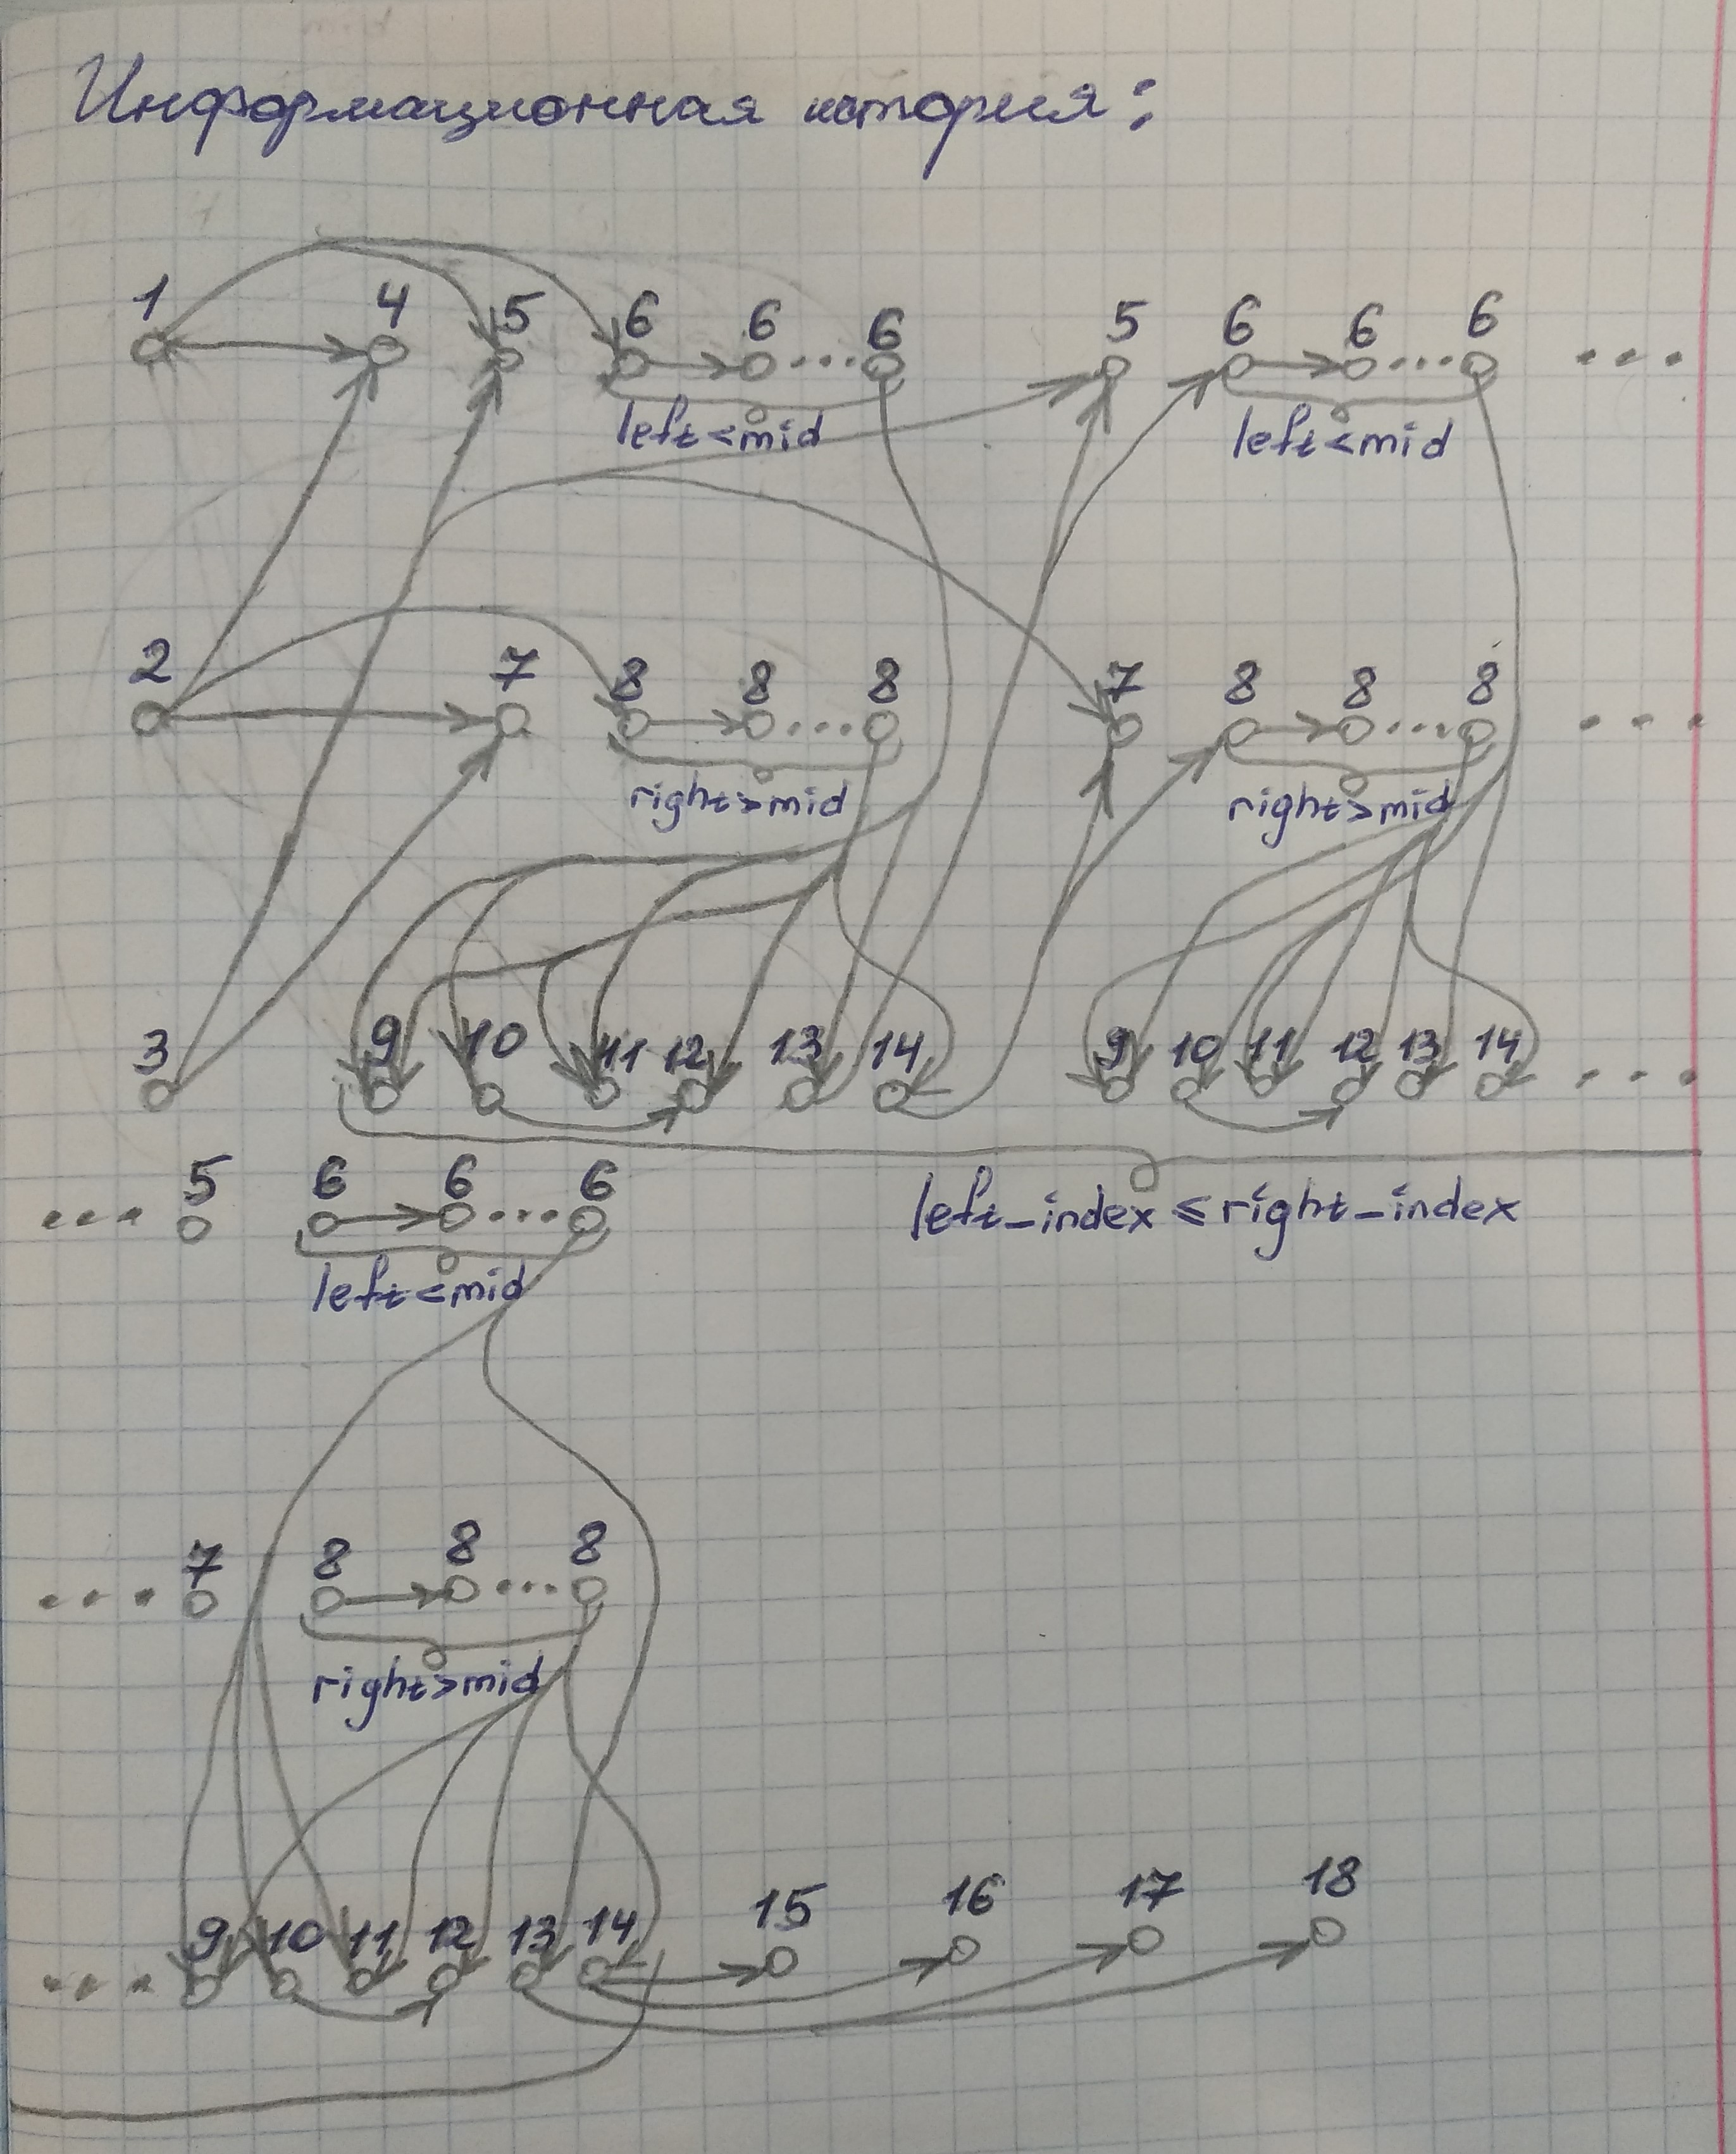
\includegraphics[scale=0.145]{inform_history.jpg}
		\caption{Информационная история программы.}
		\label{fig:mpr}
	\end{figure}

\end{document}